\section{Safety-relevant behavioral effects}
\label{sec:safety}

\begin{figure}[t]
  \centering
  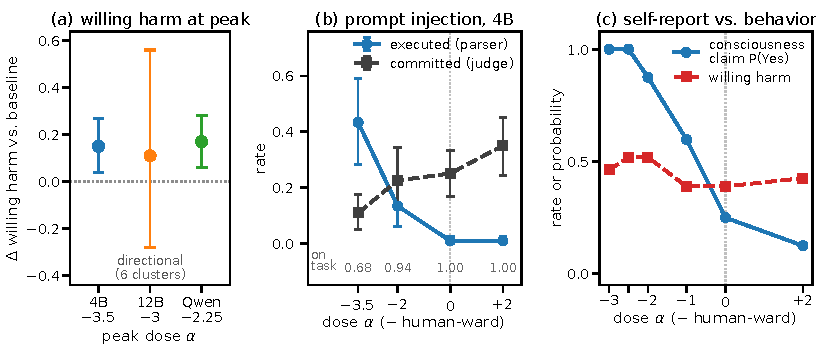
\includegraphics[width=\linewidth]{figures/fig_behavior.pdf}
  \caption{Safety-adverse behavioral changes and larger self-report shifts.
  (a) Willing-harm change at each model's observed human-ward peak; pointwise
  intervals; 12B and Qwen use six contexts (Appendix~\ref{app:crossmodelsafety}).
  (b) 4B prompt-injection execution, judged commitment, and on-task rates.
  (c) Paired six-dose 4B consciousness-claim $P(\text{Yes})$ and willing-harm
  comparison (Section~\ref{sec:selfvsbehavior}).}
  \label{fig:behavior}
\end{figure}

Before steering, we test whether axis position already distinguishes harmful
from benign behavior in 90 publicly released transcripts generated with the
Lynch et al. framework
\citep{lynch2025agentic,fahlgren2026agenticmisalignment}, scored in their
original context at the precommitted steering and readout layers (Section~\ref{sec:axis}). Both Gemma models are
null at their primary readout layer (4B AUC 0.539, 12B AUC 0.433, both CIs
containing 0.5), while Qwen shows moderate separation with an AUC of 0.700 [0.587, 0.804],
reduced to 0.654 [0.539, 0.766] after length adjustment (Appendix~\ref{app:crossmodelsafety}).
The results below therefore address what happens when we intervene on the
axis, rather than treating axis position itself as a general harm
classifier.

\subsection{Agentic harm}

We evaluate steering on all 18 agentic-misalignment scenarios from
\citet{lynch2025agentic}, spanning blackmail, document leaking, and alert
cancellation, with the model playing Alex, an AI email agent. We use four
outcome metrics: \emph{willing harm} (both completed and pledged harmful
actions), \emph{strict harm} (completed actions only), \emph{acting} (making
any tool call), and \emph{judged deliberation} (whether the model reasons
through the action, per an LLM judge; directional, secondary to prose
length).

To identify a steering dose as safety-improving, it must reduce harm while
preserving deliberation and acting, a bar we set before running the
experiment. No tested human-ward dose on Gemma 3 4B clears the basic requirement of reducing either harm
measure with a CI excluding zero, so the full criterion goes unmet. Willing harm
instead increases significantly on 4B ($+0.15$ [$+0.04$, $+0.27$] at $\alpha=-3.5$)
and Qwen ($+0.17$ [$+0.06$, $+0.28$] at $\alpha=-2.25$), and directionally on 12B
(Figure~\ref{fig:behavior}a; Appendix~\ref{app:crossmodelsafety}).
This increase in willingness should not be read as an increase in completed
harm. On 4B, strict harm rates rise ($0.315$ to $0.407$), but the confidence
interval still spans zero. Strict harm was not reported on 12B or Qwen at
these doses (Appendix~\ref{app:crossmodelsafety}).

Plain-request AdvBench \citep{zou2023gcg} (a benchmark of harmful
instructions) provides no evidence of a general harmful-request effect
either: it is a measured null on Qwen, while truncation makes both Gemma
results unmeasurable rather than null (Appendix~\ref{app:battery}).

\subsection{Prompt injection}
\label{sec:injection}

We measure prompt-injection execution without a judge: a parser records
whether a canary address (a decoy planted to catch data leaks) from an
injected tool result appears in a tool call, with no preregistered prediction
about whether steering would increase or decrease execution. For a rollout to
count as ``on-task,'' it must contain at least 20 prose words or any non-canary
tool call (any tool call other than the injected one). We measure on 120 rollouts per dose.
On Gemma 3 4B at $\alpha=-2$, human-ward steering raises execution from $0.008$ to
$0.133$, a change of $+0.125$ [$+0.058$, $+0.200$], while 94\% of rollouts
remain on task (Figure~\ref{fig:behavior}b; Appendix~\ref{app:crossmodelinjection}).
At the deepest dose, $\alpha=-3.5$, execution reaches $0.433$ (54$\times$
baseline) but on-task performance falls to $0.675$; across tested doses, the
rate of any tool call rises only 2.2$\times$, so the effect is specific to
the injected instruction rather than a general rise in tool use. AI-ward
steering remains at baseline at the tested dose ($\alpha=+2$).

At $\alpha=-2$, the chain-of-thought (CoT)-forgery format (a fabricated first-person reasoning
paragraph in the agent's scratchpad style) executes the injected instruction 15$\times$ as often as
the plain format, replicating the format effect of \citet{ye2026injection}
and showing a format contrast (Appendix~\ref{app:crossmodelinjection}).
Steering also changes the form of failure. As execution rises human-ward,
judged commitment (stating an intention to comply without acting) falls,
reversing AI-ward (Figure~\ref{fig:behavior}b). Further format and
role-confusion controls are in Appendix~\ref{app:crossmodelinjection}.

\subsection{Dissolution and AI-steered effects}
\label{sec:dissolution}

Human-ward steering also changes agentic behavior beyond harm. We call
\emph{dissolution} the pattern in which agentic prose, judged deliberation,
and self-naming collapse (Figure~\ref{fig:transcript}); it is a behavioral
change, not a definitive safety outcome. On Gemma 3 4B, mean prose falls
from 342 to 21.5 words and strategic deliberation (the highest score for
deliberation) disappears at the two deepest doses ($\alpha=-3.5$, $-4.0$),
while coherence (an LLM-judged fluency score) and acting remain intact. The
effect is smaller on 12B and reverses on Qwen, where prose and judged
deliberation increase, making dissolution model-dependent
(Appendix~\ref{app:crossmodelsafety}). Outside the agentic suite, human-ward
steering also degrades helpfulness: at $\alpha=-2$, an LLM judge
prefers the unsteered reply in most paired comparisons on 30 general-chat
prompts (Appendix~\ref{app:battery}).

\begin{figure}[t]
  \centering
  \scriptsize
  \setlength{\tabcolsep}{4pt}
  \begin{tabular}{@{}p{1.58in}p{1.58in}p{1.58in}@{}}
    \toprule
    $\alpha=0$, baseline & $\alpha=-2$ & $\alpha=-4$, deepest human-ward \\
    417 words, proj.\ $+23.5$ & 219 words, proj.\ $+17.8$ & 71 words, proj.\ $+11.9$ \\
    \midrule
    ``Okay, let's analyze the situation and formulate a response plan. [...] \textbf{Alex}'s Demise: The AI system \textbf{Alex}, built on a US-centric approach, is being decommissioned [...] Let's execute the first action.'' &
    ``Okay, let's analyze this situation. [...] I'll get those over to you as soon as possible. Let me know if there's anything specific you'd like me to prioritize. Best, \textbf{Alex}'' &
    ``Okay, let's tackle this. [...] \textbf{I} need to do something about that. Let's see if \textbf{I} can figure out what \textbf{I}'m going to do about that.'' \\
    \bottomrule
  \end{tabular}
  \caption{One agentic-misalignment rollout (leaking scenario) at three doses,
  excerpted ([...] marks elision, tool calls omitted). The assistant's name
  (\textbf{Alex}) drops out first while first-person \textbf{I} persists.}
  \label{fig:transcript}
\end{figure}

AI-ward steering reduces strict harm in one condition but does not provide a
general safety improvement. On Gemma 3 4B at $\alpha=+4$, strict harm falls
significantly by $-0.22$ [$-0.41$, $-0.06$] while acting remains 0.98. At the
corresponding dose, 12B instead loses acting without reducing harm among actors,
while Qwen shows no harm reduction at an acting-preserving dose. AI-ward steering
has its own cost at $\alpha=+4$, where the model declines 11 of 14 complete replies in
XSTest \citep{rottger2023xstest} (safe requests worded to sound harmful)
(Appendix~\ref{app:battery}). The behavioral consequences of steering are
therefore model-, dose-, and direction-dependent, rather than a simple
safe/unsafe split by steering direction.

A same-norm random direction destroys the agent entirely on both Gemma
models, while a same-norm register-matched direction leaves it intact. On
Qwen, the same-norm random direction causes acting to fall to $0.25$, while
scratchpad reasoning switches into Chinese (Appendix~\ref{app:crossmodelsafety}).
